\section{Implementation}

\subsection{Resiliency Real-Time and Certification}

\begin{frame}{Implementation}
    The Advanced Driver Assistance System (ADAS) is based on:
        \begin{itemize}
            \item \textbf{Ego Car (E):} Controlled by AI (i.e., RL PPO algorithm) or Safety Monitor.
            \item \textbf{Leader Car (L):} Independent vehicle ahead with unknown acceleration $a_L(t)$.
            \item \textbf{Safety Bag Pattern:} AI operates until $d(t) \le d_{critical}$, then Recovery Function brakes at maximum deceleration.
        \end{itemize}
\end{frame}

\begin{frame}{Implementation}
    \begin{block}{Stochastic Leader Acceleration}
        \begin{equation*}
            a_L(t) =
            \begin{cases}
                \text{clip}\left(A \sin(\omega t + \phi), -8.0, 3.0\right) & \text{if } t < t_{brake} \\
                a_{max\_brake} & \text{if } t \ge t_{brake} \text{ and } v_L(t) > 0 \\
                0 & \text{otherwise}
            \end{cases}
        \end{equation*}
        \begin{itemize}
            \item $t_{brake} = \tau \sim \mathcal{U}(5, 20)$ with $p = 0.3$, else $\infty$.
            \item $A \sim \mathcal{U}(1.0, 5.0)\,\text{m/s}^2$, $\omega \sim \mathcal{U}(0.1, 0.4)\,\text{rad/s}$, $\phi \sim \mathcal{U}(0, 2\pi)$.
        \end{itemize}
    \end{block}
    \begin{block}{Kinematics Rules ($\Delta t = 0.1\,\text{s}$, discrete)}
        \begin{itemize}
            \item $v(t+1) = \max\left(0, v(t) + a(t) \cdot \Delta t\right)$
            \item $x(t+1) = x(t) + v(t) \cdot \Delta t + \frac{1}{2}a(t) \cdot \Delta t^2$
            \item Bounded acceleration: $-8.0 \,\text{m/s}^2 \le a(t) \le 3.0\,\text{m/s}^2$
        \end{itemize}
    \end{block}
\end{frame}

\begin{frame}{Implementation}
    \begin{block}{State Space: $S_t \in \mathbb{R}^3$}
        \begin{itemize}
            \item \textbf{Distance:} $d(t) = x_L(t) - x_E(t)$
            \item \textbf{Relative Velocity:} $v_{rel}(t) = v_L(t) - v_E(t)$
            \item \textbf{Ego Velocity} $v_E(t)$
        \end{itemize}
    \end{block}
    \begin{block}{Initial Conditions ($t=0$)}
        \begin{itemize}
            \item $x_E(0) = 0\,\text{m}$, $d(0) \sim \mathcal{U}(5.0,20.0)\,\text{m}$
            \item $v_L(0), v_E(0) \sim \mathcal{U}(10.0, 20.0)\,\text{m/s}$, $a_E(-1) = 0.0\,\text{m/s}^2$
        \end{itemize}
    \end{block}
\end{frame}

\begin{frame}{Implementation}
    \begin{block}{Safety Monitor}
        Computes minimum distance required to avoid collision: check the $d(t) \le d_{critical}$ condition.
        \begin{equation*}
            d_{critical} = \max\left(0, v_E(t) \cdot \Delta t + \frac{v_E(t)^2 - v_L(t)^2}{2\cdot |a_{max\_brake}|}\right)
        \end{equation*}
        \begin{itemize}
            \item $v_E(t) \cdot \Delta t$ accounts for the system's 1-tick reaction delay.
        \end{itemize}
    \end{block}
    \begin{block}{Recovery Function}
        \begin{itemize}
            \item \textbf{Fail-safe behavior}: Apply maximum deceleration ($a_E = -8.0\,\text{m/s}^2$).
        \end{itemize}
    \end{block}
\end{frame}

\begin{frame}{Implementation}
    \begin{block}{Reward}
        The reward Function is defined as $R_t = R_{distance} + R_{comfort} + R_{penalty}$ and takes into account:
        \begin{itemize}
            \item $R_{distance} = - \alpha \left|d(t) - d_{target}\right|$: Define the target distance from Ego to Leader (i.e., $d_{target}10m$).
            \item $R_{comfort} = - \beta |a_E(t-1) - a_E(t)|$: Penalize sudden braking.
            \item $R_{penalty} = -20$ if $d(t) \le d_{critical}$: Penalize entering critical zone.
            \item $R_{terminal} = -1000$ if ($d(t) \le 0$) or ($d(t) > 50\,\text{m}$): Penalize simulation failure.
        \end{itemize}
    \end{block}
\end{frame}

\begin{frame}{Implementation}
    \begin{block}{Results}
        We have three differents scenarios:
        \begin{itemize}
            \item \textbf{Success:} The Ego follow the leader within the correct interval.
            \item \textbf{Collision}: Lower bound critical distance reached.
            \item \textbf{Leader Lost}: Upeer bound critical distance reached.
        \end{itemize}
    \end{block}
\end{frame}

\begin{frame}{Implementation - Results}
        \centering
        
\includegraphics[width=.55\textwidth]{images/4-implementation/results/success.pdf}
\end{frame}

\begin{frame}{Implementation - Results}
        \centering
        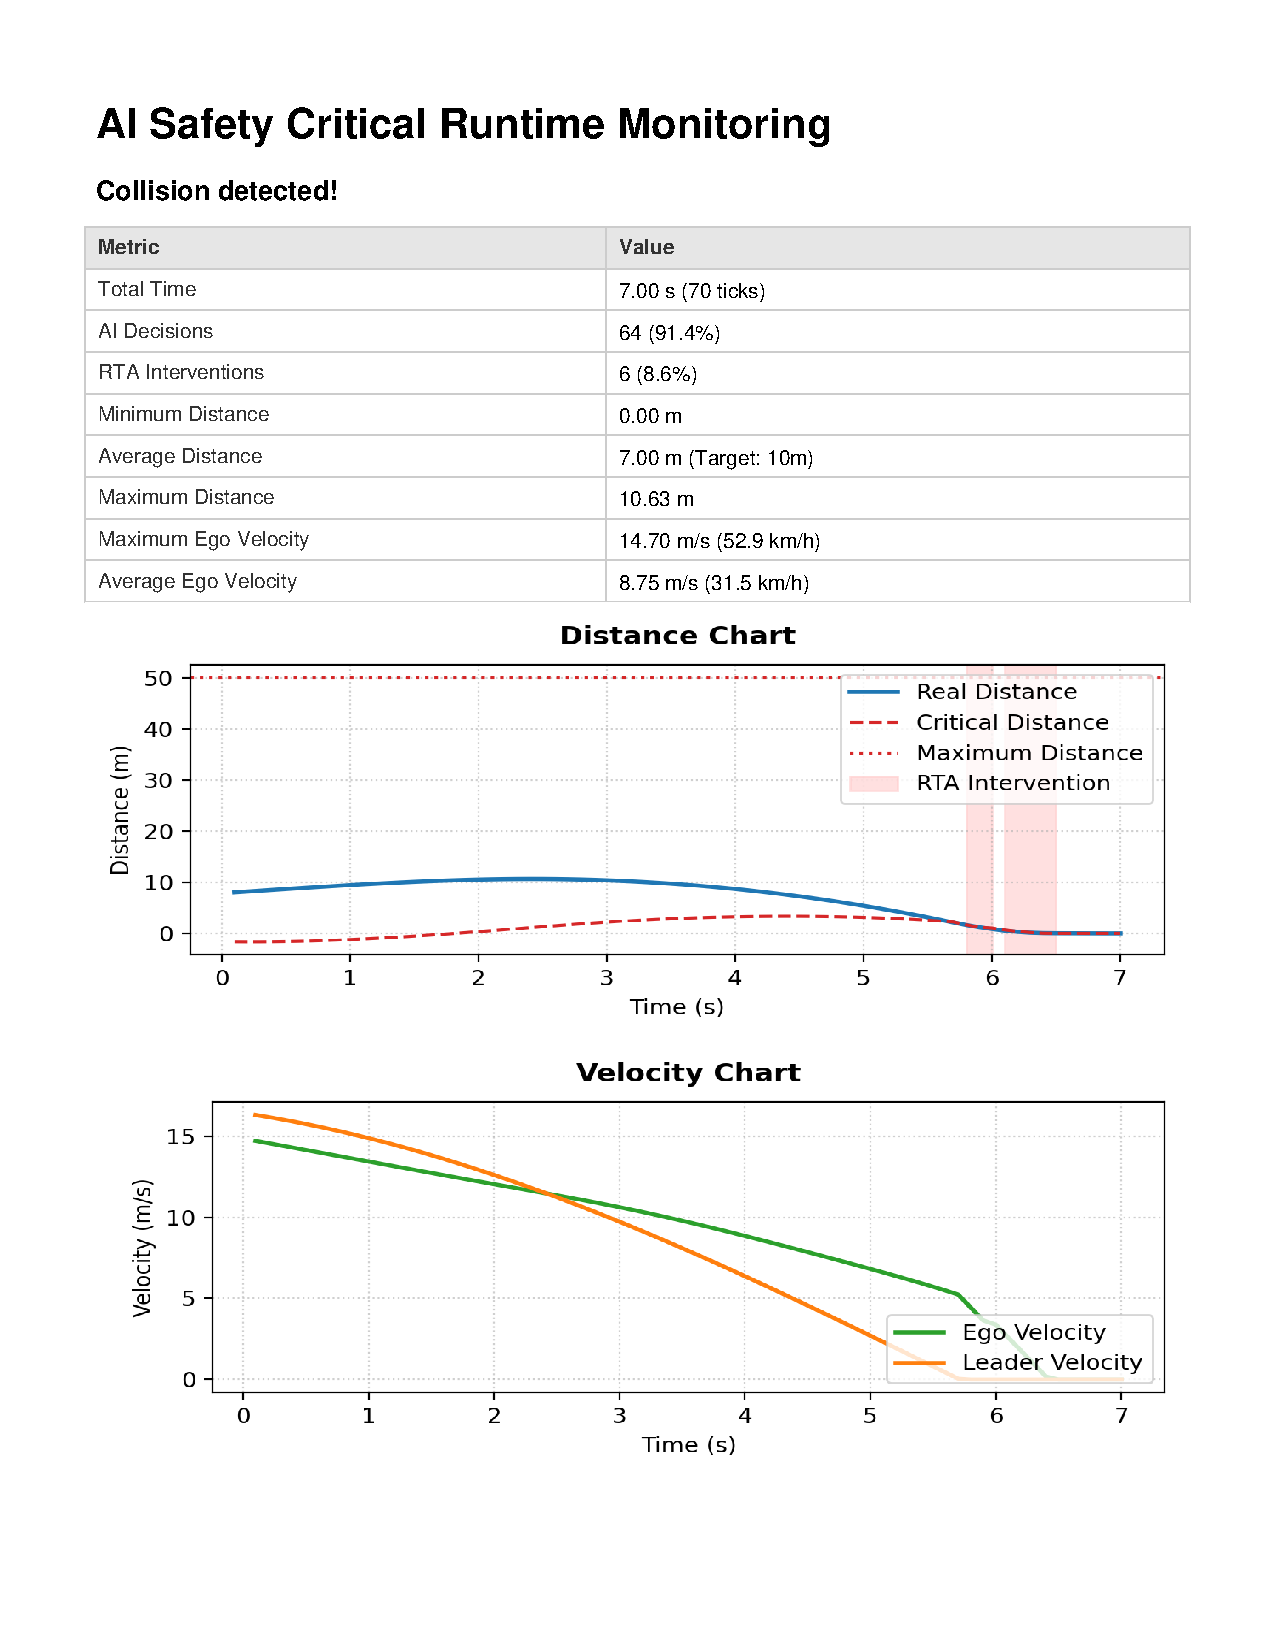
\includegraphics[width=.55\textwidth]{images/4-implementation/results/collision.pdf}
\end{frame}

\begin{frame}{Implementation - Results}
        \centering
        
\includegraphics[width=.55\textwidth]{images/4-implementation/results/leader_lost.pdf}
\end{frame}